  \documentclass[oneside]{book}
%\documentclass[12pt,]{book}

\usepackage{lmodern}
\usepackage{setspace}
\setstretch{2}
\usepackage{amssymb,amsmath}
\usepackage{ifxetex,ifluatex}
\usepackage{fixltx2e} % provides \textsubscript
\ifnum 0\ifxetex 1\fi\ifluatex 1\fi=0 % if pdftex
  \usepackage[T1]{fontenc}
  \usepackage[utf8]{inputenc}
\else % if luatex or xelatex
  \ifxetex
    \usepackage{xltxtra,xunicode}
  \else
    \usepackage{fontspec}
  \fi
  \defaultfontfeatures{Ligatures=TeX,Scale=MatchLowercase}


\fi
% use upquote if available, for straight quotes in verbatim environments
\IfFileExists{upquote.sty}{\usepackage{upquote}}{}
% use microtype if available
\IfFileExists{microtype.sty}{%
\usepackage{microtype}
\UseMicrotypeSet[protrusion]{basicmath} % disable protrusion for tt fonts
}{}
\usepackage[a4paper, left=1.18in, right=1.18in, top=1.18in, bottom=0.787in]{geometry}
\usepackage[unicode=true]{hyperref}
\hypersetup{
            pdftitle={臺大論文模板},
            pdfauthor={廖永賦},
            pdfborder={0 0 0},
            breaklinks=true}
\urlstyle{same}  % don't use monospace font for urls
\usepackage{color}
\usepackage{fancyvrb}
\newcommand{\VerbBar}{|}
\newcommand{\VERB}{\Verb[commandchars=\\\{\}]}
\DefineVerbatimEnvironment{Highlighting}{Verbatim}{commandchars=\\\{\}}
% Add ',fontsize=\small' for more characters per line
\usepackage{framed}
\definecolor{shadecolor}{RGB}{248,248,248}
\newenvironment{Shaded}{\begin{snugshade}}{\end{snugshade}}
\newcommand{\KeywordTok}[1]{\textcolor[rgb]{0.13,0.29,0.53}{\textbf{#1}}}
\newcommand{\DataTypeTok}[1]{\textcolor[rgb]{0.13,0.29,0.53}{#1}}
\newcommand{\DecValTok}[1]{\textcolor[rgb]{0.00,0.00,0.81}{#1}}
\newcommand{\BaseNTok}[1]{\textcolor[rgb]{0.00,0.00,0.81}{#1}}
\newcommand{\FloatTok}[1]{\textcolor[rgb]{0.00,0.00,0.81}{#1}}
\newcommand{\ConstantTok}[1]{\textcolor[rgb]{0.00,0.00,0.00}{#1}}
\newcommand{\CharTok}[1]{\textcolor[rgb]{0.31,0.60,0.02}{#1}}
\newcommand{\SpecialCharTok}[1]{\textcolor[rgb]{0.00,0.00,0.00}{#1}}
\newcommand{\StringTok}[1]{\textcolor[rgb]{0.31,0.60,0.02}{#1}}
\newcommand{\VerbatimStringTok}[1]{\textcolor[rgb]{0.31,0.60,0.02}{#1}}
\newcommand{\SpecialStringTok}[1]{\textcolor[rgb]{0.31,0.60,0.02}{#1}}
\newcommand{\ImportTok}[1]{#1}
\newcommand{\CommentTok}[1]{\textcolor[rgb]{0.56,0.35,0.01}{\textit{#1}}}
\newcommand{\DocumentationTok}[1]{\textcolor[rgb]{0.56,0.35,0.01}{\textbf{\textit{#1}}}}
\newcommand{\AnnotationTok}[1]{\textcolor[rgb]{0.56,0.35,0.01}{\textbf{\textit{#1}}}}
\newcommand{\CommentVarTok}[1]{\textcolor[rgb]{0.56,0.35,0.01}{\textbf{\textit{#1}}}}
\newcommand{\OtherTok}[1]{\textcolor[rgb]{0.56,0.35,0.01}{#1}}
\newcommand{\FunctionTok}[1]{\textcolor[rgb]{0.00,0.00,0.00}{#1}}
\newcommand{\VariableTok}[1]{\textcolor[rgb]{0.00,0.00,0.00}{#1}}
\newcommand{\ControlFlowTok}[1]{\textcolor[rgb]{0.13,0.29,0.53}{\textbf{#1}}}
\newcommand{\OperatorTok}[1]{\textcolor[rgb]{0.81,0.36,0.00}{\textbf{#1}}}
\newcommand{\BuiltInTok}[1]{#1}
\newcommand{\ExtensionTok}[1]{#1}
\newcommand{\PreprocessorTok}[1]{\textcolor[rgb]{0.56,0.35,0.01}{\textit{#1}}}
\newcommand{\AttributeTok}[1]{\textcolor[rgb]{0.77,0.63,0.00}{#1}}
\newcommand{\RegionMarkerTok}[1]{#1}
\newcommand{\InformationTok}[1]{\textcolor[rgb]{0.56,0.35,0.01}{\textbf{\textit{#1}}}}
\newcommand{\WarningTok}[1]{\textcolor[rgb]{0.56,0.35,0.01}{\textbf{\textit{#1}}}}
\newcommand{\AlertTok}[1]{\textcolor[rgb]{0.94,0.16,0.16}{#1}}
\newcommand{\ErrorTok}[1]{\textcolor[rgb]{0.64,0.00,0.00}{\textbf{#1}}}
\newcommand{\NormalTok}[1]{#1}
\usepackage{longtable,booktabs}
% Fix footnotes in tables (requires footnote package)
\IfFileExists{footnote.sty}{\usepackage{footnote}\makesavenoteenv{long table}}{}
\let\oldhref=\href
% Make links footnotes instead of hotlinks:
\renewcommand{\href}[2]{#2\footnote{\url{#1}}}
\IfFileExists{parskip.sty}{%
\usepackage{parskip}
}{% else
\setlength{\parindent}{0pt}
\setlength{\parskip}{6pt plus 2pt minus 1pt}
}
\setlength{\emergencystretch}{3em}  % prevent overfull lines
\providecommand{\tightlist}{%
  \setlength{\itemsep}{0pt}\setlength{\parskip}{0pt}}
\setcounter{secnumdepth}{5}

% set default figure placement to htbp
\makeatletter
\def\fps@figure{htbp}
\makeatother

\usepackage{pdfpages}
\usepackage{titlesec}
\usepackage{titletoc}
\usepackage{booktabs}
\usepackage{apptools}
\usepackage{float}
\usepackage[section]{placeins}

\usepackage[heading, fontset = none]{ctex}
\ctexset{appendix/name={\appendixname\space}}
%\usepackage[UTF8, heading = true, fontset = none]{ctex}%
%\ctexset {

%    fontset = none,
%    appendixname = "附錄",

    %chapter/name = {第,章},
    %chapter/titleformat = \chaptertitleformat,
    %section/name = {\S},


%    appendix = {
%        numbering = true,
%        name = {附錄}
%        }
%}



%中文自動換行
\XeTeXlinebreaklocale "zh"
%文字的彈性間距
\XeTeXlinebreakskip = 0pt plus 1pt



\renewcommand{\figurename}{圖}
\renewcommand{\tablename}{表}
\renewcommand{\contentsname}{目錄}
\renewcommand{\listfigurename}{圖目錄}
\renewcommand{\listtablename}{表目錄}
\renewcommand{\appendixname}{附錄}
%\renewcommand{\bibname}{參考資料}

\title{臺大論文模板}
\author{廖永賦}
\date{November 9, 2018}


\usepackage{fontspec}
%使用xeCJK,其他的還有CJK或是xCJK
\usepackage{xeCJK}
\usepackage{bm}

% Set the default fonts
  \setmainfont{Liberation Serif} % Times New Roman  %Liberation Serif

                        \setCJKmainfont[AutoFakeBold=2.5, AutoFakeSlant=.3]{AR PL KaitiM Big5} %標楷體 %AR PL KaitiM Big5
            %\setCJKmainfont[AutoFakeBold=1,AutoFakeSlant=.4]{BiauKai}
            


% IPA support (Works with linguisticsdown)
  \newfontfamily\ipa{Doulos SIL} % Font for IPA symbols
  \DeclareTextFontCommand{\ipatext}{\ipa}


\usepackage{xcolor}
\usepackage{transparent}
\usepackage[printwatermark]{xwatermark}

  \newwatermark*[allpages,xpos=6.1725cm,ypos=10.5225cm,scale=0.5]{
\includegraphics{watermark.pdf}}



\usepackage{amsthm}
\newtheorem{theorem}{Theorem}[chapter]
\newtheorem{lemma}{Lemma}[chapter]
\theoremstyle{definition}
\newtheorem{definition}{定義}[chapter]
\newtheorem{corollary}{Corollary}[chapter]
\newtheorem{proposition}{Proposition}[chapter]
\theoremstyle{definition}
\newtheorem{example}{例}[chapter]
\theoremstyle{definition}
\newtheorem{exercise}{Exercise}[chapter]
\theoremstyle{remark}
\newtheorem*{remark}{Remark}
\newtheorem*{solution}{Solution}
\let\BeginKnitrBlock\begin \let\EndKnitrBlock\end
\begin{document}



\includepdf[pages={1}, scale=1]{front_matter/front_matter.pdf}

\clearpage
\pagenumbering{roman}

\phantomsection
\addcontentsline{toc}{chapter}{口試委員會審定書}

\includepdf[pages={1}, scale=1]{certification-scan.pdf}

\phantomsection
\addcontentsline{toc}{chapter}{誌謝}

\includepdf[pages={3}, scale=1]{front_matter/front_matter.pdf}


\phantomsection
\addcontentsline{toc}{chapter}{中文摘要}

\includepdf[pages={4}, scale=1]{front_matter/front_matter.pdf}

\phantomsection
\addcontentsline{toc}{chapter}{英文摘要}

\includepdf[pages={5}, scale=1]{front_matter/front_matter.pdf}


{
\setcounter{tocdepth}{1}
\tableofcontents
%\phantomsection
%\addcontentsline{toc}{chapter}{\contentsname}
}

\newpage

\listoftables
\phantomsection
\addcontentsline{toc}{chapter}{\listtablename}
\newpage

\listoffigures
\phantomsection
\addcontentsline{toc}{chapter}{\listfigurename}
\newpage

% Set independent linestretch for code chunks
\let\oldShaded=\Shaded
\let\endoldShaded=\endShaded
\renewenvironment{Shaded}{
      \begin{spacing}{1.5}\begin{oldShaded}
    }
  {
  \end{oldShaded}
  \end{spacing}
  }

\clearpage
\pagenumbering{arabic}

\chapter{安裝}\label{install}

\begin{Shaded}
\begin{Highlighting}[]
\NormalTok{devtools}\OperatorTok{::}\KeywordTok{install_github}\NormalTok{(}\StringTok{"liao961120/ntuthesis"}\NormalTok{)}
\end{Highlighting}
\end{Shaded}

\section{LaTeX}\label{latex}

若已有管理、安裝 LaTeX 套件經驗者,可忽略。

若電腦尚未安裝 LaTeX,可安裝 R 的 tinytex 套件:

\begin{Shaded}
\begin{Highlighting}[]
\KeywordTok{install.packages}\NormalTok{(}\StringTok{'tinytex'}\NormalTok{)}
\NormalTok{tinytex}\OperatorTok{::}\KeywordTok{install_tinytex}\NormalTok{()}
\end{Highlighting}
\end{Shaded}

在輸出 R Markdown 時,tinytex 會自動安裝缺少的 LaTeX
套件。因此,第一次輸出 PDF 可能會需要一些時間。

\chapter{輸出論文}\label{export-thesis}

\section{匯入論文模板}\label{import-template}

開啟 RStudio,選取左上方 \texttt{File} \textgreater{} \texttt{New\ File}
\textgreater{} \texttt{R\ Markdown}:

\begin{Shaded}
\begin{Highlighting}[]
\ControlFlowTok{if}\NormalTok{ (knitr}\OperatorTok{::}\KeywordTok{is_html_output}\NormalTok{()) \{}
\NormalTok{  knitr}\OperatorTok{::}\KeywordTok{include_graphics}\NormalTok{(}\StringTok{"figs/rmd-template.gif"}\NormalTok{)}
\NormalTok{\} }\ControlFlowTok{else}\NormalTok{ \{}
\NormalTok{  knitr}\OperatorTok{::}\KeywordTok{include_graphics}\NormalTok{(}\StringTok{"figs/rmd-template.png"}\NormalTok{)}
\NormalTok{\}}
\end{Highlighting}
\end{Shaded}

\begin{figure}[H]

{\centering 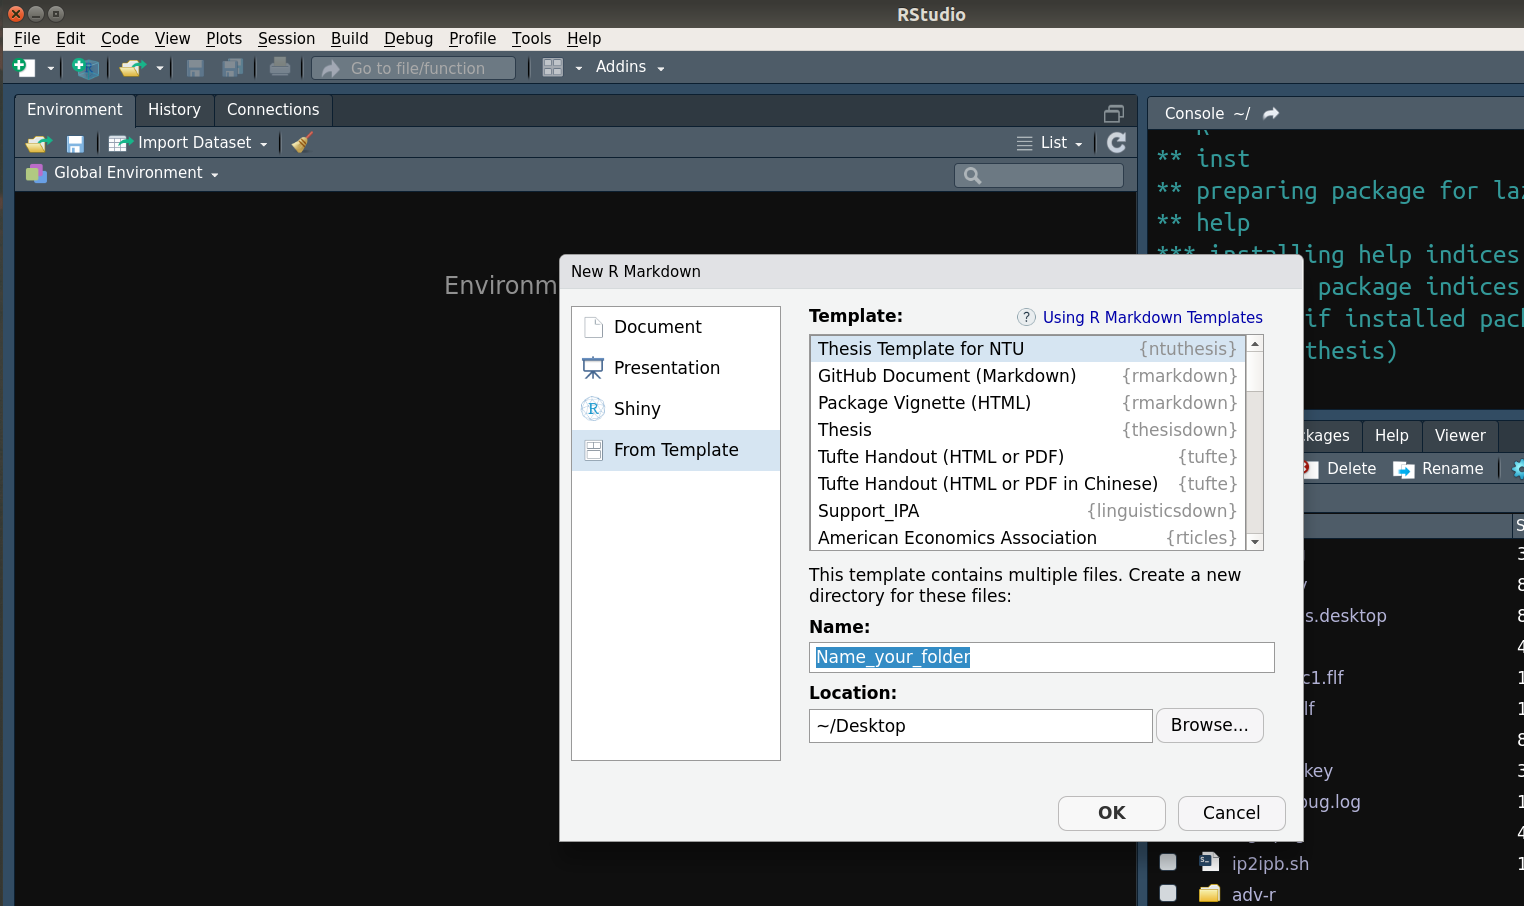
\includegraphics[width=1\linewidth]{figs/rmd-template} 

}

\caption{透過 RStudio 匯入論文模板}\label{fig:unnamed-chunk-2}
\end{figure}

或是直接在 console 執行:

\begin{Shaded}
\begin{Highlighting}[]
\NormalTok{rmarkdown}\OperatorTok{::}\KeywordTok{draft}\NormalTok{(}\StringTok{"project_name"}\NormalTok{,}
                 \DataTypeTok{template =} \StringTok{"ntu_bookdown"}\NormalTok{,}
                 \DataTypeTok{package =} \StringTok{"ntuthesis"}\NormalTok{)}
\end{Highlighting}
\end{Shaded}

接著需要將該資料夾變更為 bookdown 專案。這可以用 RStudio 左上方
\texttt{File} \textgreater{} \texttt{New\ Project} \textgreater{}
\texttt{Existing\ Directory} 達成,或直接使用下方指令(working dir
需是專案資料夾):

\begin{Shaded}
\begin{Highlighting}[]
\NormalTok{ntuthesis}\OperatorTok{::}\KeywordTok{init_proj}\NormalTok{()  }\CommentTok{# init working dir as proj.}
\end{Highlighting}
\end{Shaded}

詳細的檔案結構,見 \ref{dir-structure}。

\section{編輯封面}\label{edit-front-matter}

在\texttt{\_person-info.yml}輸入個人資料後,執行:

\begin{Shaded}
\begin{Highlighting}[]
\NormalTok{ntuthesis}\OperatorTok{::}\KeywordTok{comp_front}\NormalTok{()}
\end{Highlighting}
\end{Shaded}

即會在 \texttt{front-matter/}
生成封面所需的檔案。以使用者的角度而言,除了
\texttt{front-matter/certification.pdf} 以外,\texttt{front-matter/}
中的其它檔案不須理會。\texttt{certification.pdf}
是空白(未簽名)的「口試委員審定書」。

已簽名的「口試委員審定書」,將檔案命名為 \texttt{certification-scan.pdf}
並放在專案資料夾的最頂層。

\section{Compile 論文}\label{compile-thesis}

接著用 RStudio Build Pane 裡的 button 輸出論文:

\begin{Shaded}
\begin{Highlighting}[]
\ControlFlowTok{if}\NormalTok{ (knitr}\OperatorTok{::}\KeywordTok{is_html_output}\NormalTok{()) \{}
\NormalTok{  knitr}\OperatorTok{::}\KeywordTok{include_graphics}\NormalTok{(}\StringTok{"figs/build-button.gif"}\NormalTok{)}
\NormalTok{\} }\ControlFlowTok{else}\NormalTok{ \{}
\NormalTok{  knitr}\OperatorTok{::}\KeywordTok{include_graphics}\NormalTok{(}\StringTok{"figs/build-button.png"}\NormalTok{)}
\NormalTok{\}}
\end{Highlighting}
\end{Shaded}

\begin{figure}[H]

{\centering 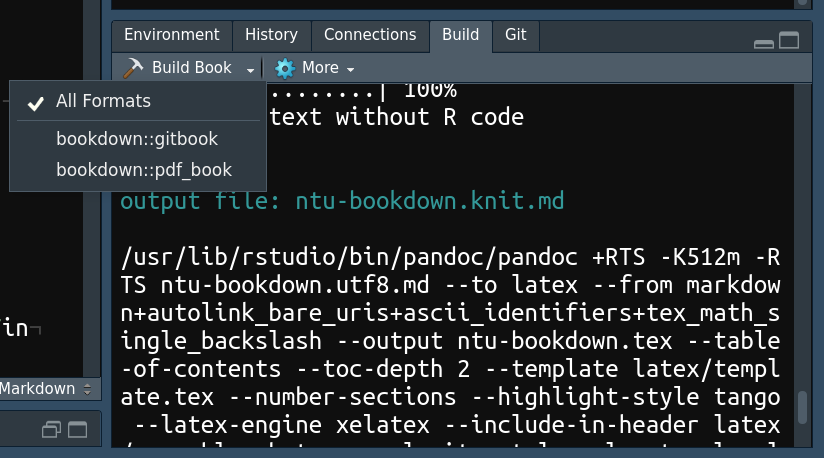
\includegraphics[width=1\linewidth]{figs/build-button} 

}

\caption{透過 RStudio 輸出論文}\label{fig:unnamed-chunk-3}
\end{figure}

或是在 console 執行下方指令:

\begin{Shaded}
\begin{Highlighting}[]
\NormalTok{bookdown}\OperatorTok{::}\KeywordTok{render_book}\NormalTok{(}\StringTok{"index.Rmd"}\NormalTok{, }\StringTok{"bookdown::gitbook"}\NormalTok{)}
\NormalTok{bookdown}\OperatorTok{::}\KeywordTok{render_book}\NormalTok{(}\StringTok{"index.Rmd"}\NormalTok{, }\StringTok{"bookdown::bookdown::pdf_book"}\NormalTok{)}
\end{Highlighting}
\end{Shaded}

如此便會在 \texttt{\_book/} 中生成完整的論文(gitbook 和 PDF 格式)。

\chapter{論文撰寫}\label{write-thesis}

\section{檔案結構}\label{dir-structure}

執行以下指令後(詳見 \ref{import-template})

\begin{Shaded}
\begin{Highlighting}[]
\NormalTok{rmarkdown}\OperatorTok{::}\KeywordTok{draft}\NormalTok{(}\StringTok{"project_name"}\NormalTok{,}
                 \DataTypeTok{template =} \StringTok{"ntu_bookdown"}\NormalTok{,}
                 \DataTypeTok{package =} \StringTok{"ntuthesis"}\NormalTok{)}
\end{Highlighting}
\end{Shaded}

即會匯入論文模板,以下是論文模板的檔案結構(已簡化)。

\begin{Shaded}
\begin{Highlighting}[]
\NormalTok{├── project_name.Rmd     }\CommentTok{# Useless, please delete it}
\NormalTok{|}
\NormalTok{├── R/                   }\CommentTok{# code chunk root dir, put R scripts and data here}
\NormalTok{├── figs/                }\CommentTok{# Put figures to include in the thesis here}
\NormalTok{|}
\NormalTok{├── index.Rmd            }\CommentTok{# Book Layout (font, watermark, biblio, ...)}
\NormalTok{├── _acknowledge.Rmd     }\CommentTok{# acknowledgement}
\NormalTok{├── _abstract-en.Rmd     }\CommentTok{# abstract}
\NormalTok{├── _abstract-zh.Rmd     }\CommentTok{# Same as above, but in Chinese}
\NormalTok{|}
\NormalTok{├── 01-intro.Rmd         }\CommentTok{# Chapter 1 content}
\NormalTok{├── 02-literature.Rmd    }\CommentTok{# Chapter 2 content}
\NormalTok{├── 03-method.Rmd        }\CommentTok{# Chapter 3 content}
\NormalTok{├── 99-references.Rmd    }\CommentTok{# Don't need to edit}
\NormalTok{├── ref.bib              }\CommentTok{# References}
\NormalTok{├── cite-style.csl       }\CommentTok{# Citation style}
\NormalTok{|}
\NormalTok{├── _bookdown.yml        }\CommentTok{# label names in gitbook; Rmd files order}
\NormalTok{├── _output.yml          }\CommentTok{# preamble, pandoc args, cite-pkg}
\NormalTok{|}
\NormalTok{├── watermark.pdf        }\CommentTok{# 臺大浮水印 (PDF 右上角)}
\NormalTok{├── _person-info.yml      }\CommentTok{# Info to generate front matter}
\NormalTok{├── certification-scan.pdf  }\CommentTok{# 已簽名'口試委員審查書'}
\NormalTok{└── front_matter}
\NormalTok{    └── certification.pdf   }\CommentTok{# 空白'口試委員審查書'}
\end{Highlighting}
\end{Shaded}

\section{\texorpdfstring{\texttt{index.Rmd}}{index.Rmd}}\label{index-rmd}

\texttt{index.Rmd} 是設定論文內文格式的地方,包含 yaml 以及 R setup code
chunk。此模板將 code chunk 預設的 working directory 改成
\texttt{R/}\footnote{預設是 Rmd 檔所在的位置。},如此較符合一般寫
Rscript 的邏輯\footnote{例如,使用相對路徑匯入資料時,一般會以 Rscript
  所在的位置作為基準。}。若要更改此設定,至 setup code chunk 更改
\texttt{knitr::opts\_knit\$set(root.dir=\textquotesingle{}R\textquotesingle{})}。

\section{撰寫語言}\label{write-lang}

若使用\textbf{英文}撰寫論文,需修改
\texttt{\_output.yml}、\texttt{\_bookdown.yml} 這兩個檔案的內容。

\subsection{\texorpdfstring{\texttt{\_output.yml}}{\_output.yml}}\label{output.yml}

將 \texttt{in\_header:\ latex/preamble-zh.tex} 改為
\texttt{in\_header:\ latex/preamble-en.tex}:

\begin{Shaded}
\begin{Highlighting}[]
\FunctionTok{bookdown:}\AttributeTok{:pdf_book:}
  \FunctionTok{includes:}
    \FunctionTok{in_header:}\AttributeTok{ latex/preamble-en.tex}
\end{Highlighting}
\end{Shaded}

\subsection{\texorpdfstring{\texttt{\_bookdown.yml}}{\_bookdown.yml}}\label{bookdown.yml}

\texttt{\_bookdown.yml} 中,可以對標籤的名稱進行定義。這裡的設定與 PDF
輸出無關,只與 gitbook 輸出格式有關。因此,若無需使用 gitbook
輸出,可忽略此段。

此外,\texttt{\_bookdown.yml} 亦可設定 Rmd
檔在輸出文件中的順序。若無設定,就會依序檔名排序\footnote{此模板即未進行設定,因此第一章的內容寫在
  \texttt{01-xxx.Rmd}
  就會自動排在第一。而若檔名以底線開頭(\texttt{\_})則會被忽略。更多內容詳見
  \href{https://bookdown.org/yihui/bookdown/usage.html}{bookdown}。}。

在以下設定中,可使 gitbook 輸出的章節(順序)與 PDF 不同。

\begin{Shaded}
\begin{Highlighting}[]
\FunctionTok{rmd_files:}
  \FunctionTok{html:}\AttributeTok{ }\KeywordTok{[}\StringTok{"index.Rmd"}\KeywordTok{,} \StringTok{"abstract.Rmd"}\KeywordTok{,} \StringTok{"intro.Rmd"}\KeywordTok{]}
  \FunctionTok{latex:}\AttributeTok{ }\KeywordTok{[}\StringTok{"abstract.Rmd"}\KeywordTok{,} \StringTok{"intro.Rmd"}\KeywordTok{]}
\end{Highlighting}
\end{Shaded}

\section{文獻引用}\label{bib-cite}

R Markdown 在文章中插入引用文獻的功能承繼 Pandoc。完整的使用見
\href{https://rmarkdown.rstudio.com/authoring_bibliographies_and_citations.html}{R
Markdown 官方說明} 。

此模板目前產生文獻格式的方法是依靠
\href{https://github.com/jgm/pandoc-citeproc}{Pandoc
citeproc},因此,文獻格式是依據 \texttt{cite-style.csl}\footnote{此模板提供的
  \texttt{cite-style.csl} 是 APA
  英文第六版。此外,\url{http://blog.pulipuli.info/2011/05/zoteroapa.html}
  亦有提供 APA 中文版的引用格式。需注意的是 Pandoc \textbf{不支援雙語
  csl}
  (\url{http://blog.pulipuli.info/2014/08/zoteroapa-zotero-citation-style-apa.html})。}
產生的。使用者可至 \href{https://www.zotero.org/styles}{Zotero Style
Repository} 下載所需的 csl 檔並覆蓋專案資料夾中的
\texttt{cite-style.csl}。

\subsection{\texorpdfstring{\texttt{ref.bib}}{ref.bib}}\label{ref-bib}

\texttt{.bib} 檔的產生方式可以由 Endnote, Zotero, JabRef
等書目管理軟體匯出。匯出後,將檔名命名為 \texttt{ref.bib}
放在專案資料夾\footnote{或是可以自訂檔名,並到 \texttt{index.Rmd} yaml
  中的 \texttt{bibliography:\ ref.bib} 更改 \texttt{ref.bib}
  檔名。此外,亦可使用多個 \texttt{.bib}
  檔:\texttt{bibliography:\ {[}ref1.bib,\ ref2.bib,\ ref3.bib{]}}。}。

\texttt{.bib} 內的一篇引用資料會類似:

\begin{Shaded}
\begin{Highlighting}[]
\VariableTok{@article}\NormalTok{\{}\OtherTok{leung2008}\NormalTok{,}
  \DataTypeTok{title}\NormalTok{ = \{Multicultural Experience Enhances Creativity: \{\{The\}\} When and How.\},}
  \DataTypeTok{volume}\NormalTok{ = \{63\},}
  \DataTypeTok{issn}\NormalTok{ = \{1935-990X(Electronic),0003-066X(Print)\},}
  \DataTypeTok{doi}\NormalTok{ = \{10.1037/0003-066X.63.3.169\},}
  \DataTypeTok{number}\NormalTok{ = \{3\},}
  \DataTypeTok{journaltitle}\NormalTok{ = \{American Psychologist\},}
  \DataTypeTok{date}\NormalTok{ = \{2008\},}
  \DataTypeTok{pages}\NormalTok{ = \{169-181\},}
  \DataTypeTok{keywords}\NormalTok{ = \{*Cognition,*Creativity,*Culture (Anthropological),*Experiences (Events),Multiculturalism\},}
  \DataTypeTok{author}\NormalTok{ = \{Leung, Angela Ka-yee and Maddux, William W. and Galinsky, Adam D. and Chiu, Chi-yue\}}
\NormalTok{\}}
\end{Highlighting}
\end{Shaded}

其中第一行的 \texttt{leung2008} 即為 citation key。透過
\texttt{@citekey}(\texttt{@leung2008})即可在文獻中插入
citation。匯出論文時,文末會自動產生引用的文獻。

\subsection{引用語法}\label{cite-syntax}

\href{https://github.com/crsh/citr}{\texttt{citr}}
是一個方便使用者插入引用文獻的 R 套件,讓使用者能透過 GUI 插入文獻:

\begin{Shaded}
\begin{Highlighting}[]
\ControlFlowTok{if}\NormalTok{ (knitr}\OperatorTok{::}\KeywordTok{is_html_output}\NormalTok{())\{}
\NormalTok{  knitr}\OperatorTok{::}\KeywordTok{include_graphics}\NormalTok{(}\StringTok{"figs/citr.gif"}\NormalTok{)}
\NormalTok{\} }\ControlFlowTok{else}\NormalTok{ \{}
\NormalTok{  knitr}\OperatorTok{::}\KeywordTok{include_graphics}\NormalTok{(}\StringTok{"figs/citr.png"}\NormalTok{)}
\NormalTok{\}}
\end{Highlighting}
\end{Shaded}

\begin{figure}[H]

{\centering 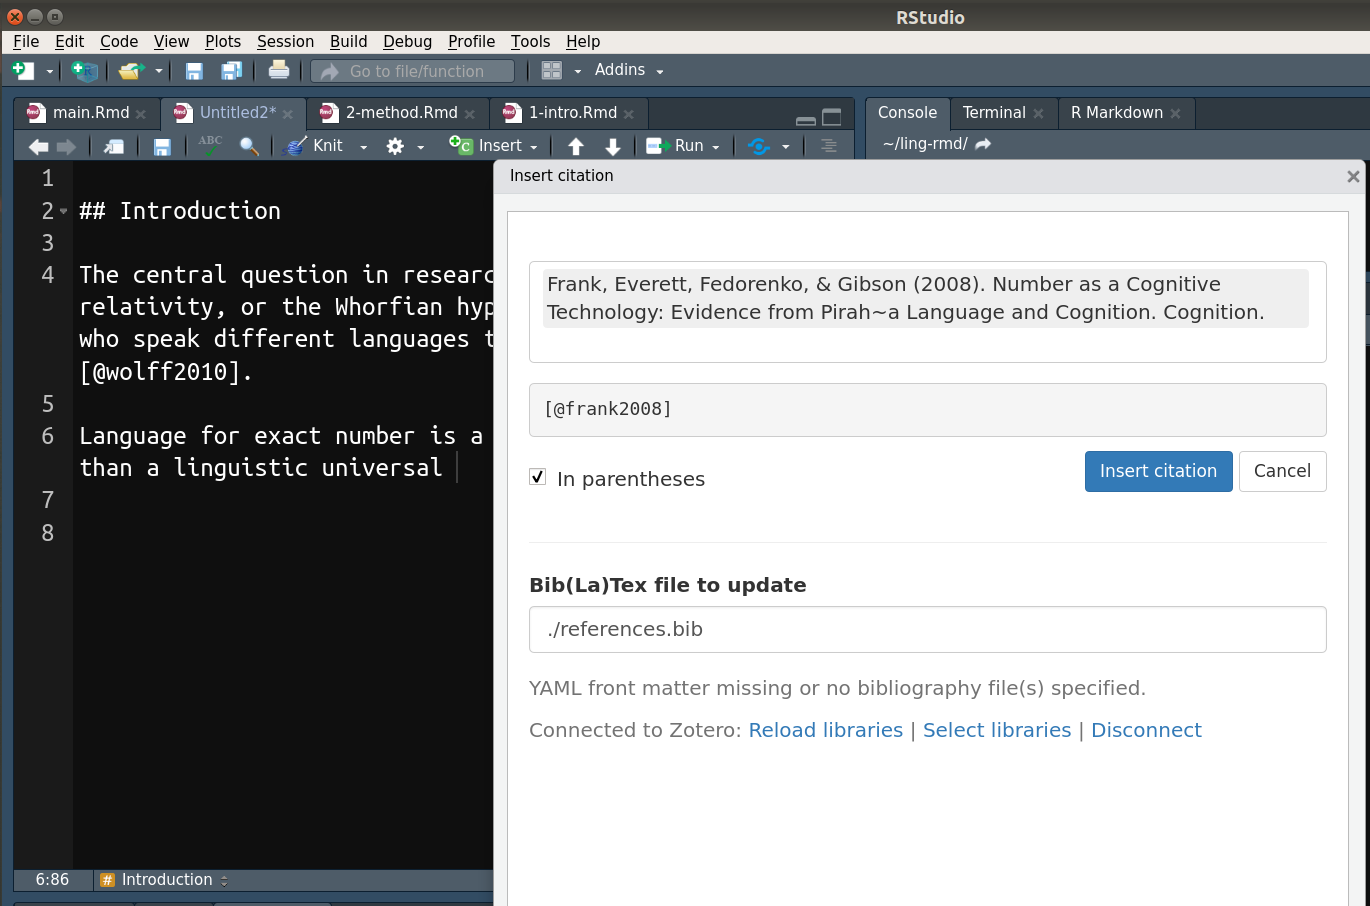
\includegraphics[width=1\linewidth]{figs/citr} 

}

\caption{使用 citr 套件插入引用文獻}\label{fig:unnamed-chunk-5}
\end{figure}

當需要更複雜的引用格式,如標示第幾頁,可以修改透過 \texttt{citr}
插入的語法:

\begin{itemize}
\tightlist
\item
  \texttt{Some\ text\ {[}@citekey{]}.}

  \begin{itemize}
  \tightlist
  \item
    Some text (Leung, Maddux, Galinsky, \& Chiu,
    \protect\hyperlink{ref-leung2008}{2008}).
  \end{itemize}
\item
  \texttt{@citekey\ Some\ text}

  \begin{itemize}
  \tightlist
  \item
    Leung et al. (\protect\hyperlink{ref-leung2008}{2008}) Some text
  \end{itemize}
\item
  \texttt{@citekey\ {[}p.\ 20{]}\ Some\ text.}

  \begin{itemize}
  \tightlist
  \item
    Leung et al. (\protect\hyperlink{ref-leung2008}{2008}, p. 20) Some
    text.
  \end{itemize}
\item
  \texttt{Some\ text\ {[}-@citekey{]}.}

  \begin{itemize}
  \tightlist
  \item
    Some text (\protect\hyperlink{ref-leung2008}{2008})
  \end{itemize}
\item
  \texttt{Some\ text\ {[}@citekey1;\ @citekey2{]}.}

  \begin{itemize}
  \tightlist
  \item
    Some text (Leung et al., \protect\hyperlink{ref-leung2008}{2008};
    黃宣範, \protect\hyperlink{ref-huangxuanfan1993}{1993}).
  \end{itemize}
\item
  Prefix \& Suffix

  \begin{itemize}
  \tightlist
  \item
    \texttt{Text\ {[}see\ @citekey1\ pp.45;\ also,\ @citekey2\ ch.\ 2{]}.}
  \item
    Text (see Leung et al., \protect\hyperlink{ref-leung2008}{2008}, p.
    45; also, 黃宣範, \protect\hyperlink{ref-huangxuanfan1993}{1993}
    ch.~2).
  \end{itemize}
\end{itemize}

\subsection{書目管理軟體}\label{ref-manager}

這裡建議使用 Zotero 加上
\href{https://retorque.re/zotero-better-bibtex/}{Better BibTeX}
擴充功能。\texttt{citr} 對 Zotero 有額外的支持,且 \textbf{Zotero
能夠控制 citation key 的格式}(例如,last name +
year),但其它書目管理軟體如 Endnote 產生的 citation key
對難以讀懂且無法更改其格式。

\subsection{多語言文獻引用}\label{multi-lang-cite}

透過 csl
排版引用格式,只能支援單一語言。例如,若將英文格式套用到中文文獻,中文文獻就會出現英文的半形逗點和句點。

多語言的引用可能可透過 LaTeX 的引用套件達成,但由於作者本人對 LaTeX
不夠熟悉,目前尚未解決此問題。若您是 LaTeX 的高手,歡迎至
\ref{latex-cite-pkg} 給我一些指教。

\chapter{語法 Cheatsheet}\label{cheatsheet}

\section{數學}\label{math}

完整內容,詳見 Bookdown
\href{https://bookdown.org/yihui/bookdown/markdown-extensions-by-bookdown.html}{Ch.
2}

\subsection{Unnumbered Equations}\label{unnumbered-equations}

\begin{Shaded}
\begin{Highlighting}[]
\KeywordTok{\textbackslash{}begin}\NormalTok{\{}\ExtensionTok{equation*}\NormalTok{\}}\SpecialStringTok{ }
\SpecialCharTok{\textbackslash{}frac}\SpecialStringTok{\{d\}\{dx\}}\SpecialCharTok{\textbackslash{}left}\SpecialStringTok{( }\SpecialCharTok{\textbackslash{}int}\SpecialStringTok{_\{a\}^\{x\} f(u)}\SpecialCharTok{\textbackslash{},}\SpecialStringTok{du}\SpecialCharTok{\textbackslash{}right}\SpecialStringTok{)=f(x)}
\KeywordTok{\textbackslash{}end}\NormalTok{\{}\ExtensionTok{equation*}\NormalTok{\} }
\end{Highlighting}
\end{Shaded}

\begin{equation*} 
\frac{d}{dx}\left( \int_{a}^{x} f(u)\,du\right)=f(x)
\end{equation*}

\subsection{Numbered Equations}\label{numbered-equations}

\begin{Shaded}
\begin{Highlighting}[]
\KeywordTok{\textbackslash{}begin}\NormalTok{\{}\ExtensionTok{equation}\NormalTok{\}}\SpecialStringTok{ }
\SpecialStringTok{  f}\SpecialCharTok{\textbackslash{}left}\SpecialStringTok{(k}\SpecialCharTok{\textbackslash{}right}\SpecialStringTok{) = }\SpecialCharTok{\textbackslash{}binom}\SpecialStringTok{\{n\}\{k\} p^k}\SpecialCharTok{\textbackslash{}left}\SpecialStringTok{(1-p}\SpecialCharTok{\textbackslash{}right}\SpecialStringTok{)^\{n-k\}}
\SpecialStringTok{  (}\SpecialCharTok{\textbackslash{}#}\SpecialStringTok{eq:bino)}
\KeywordTok{\textbackslash{}end}\NormalTok{\{}\ExtensionTok{equation}\NormalTok{\} }

\NormalTok{式 }\FunctionTok{\textbackslash{}@ref}\NormalTok{(eq:bino)}
\end{Highlighting}
\end{Shaded}

\begin{equation} 
  f\left(k\right) = \binom{n}{k} p^k\left(1-p\right)^{n-k}
  \label{eq:binom}
\end{equation}

式 \eqref{eq:binom}

\subsection{Multi-line Aligned
Equations}\label{multi-line-aligned-equations}

\begin{Shaded}
\begin{Highlighting}[]
\KeywordTok{\textbackslash{}begin}\NormalTok{\{}\ExtensionTok{equation}\NormalTok{\}}\SpecialStringTok{ }
\KeywordTok{\textbackslash{}begin}\NormalTok{\{}\ExtensionTok{split}\NormalTok{\}}
\SpecialCharTok{\textbackslash{}mathrm}\SpecialStringTok{\{Var\}(}\SpecialCharTok{\textbackslash{}hat}\SpecialStringTok{\{}\SpecialCharTok{\textbackslash{}beta}\SpecialStringTok{\}) & =}\SpecialCharTok{\textbackslash{}mathrm}\SpecialStringTok{\{Var\}((X'X)^\{-1\}X'y)}\SpecialCharTok{\textbackslash{}\textbackslash{}}
\SpecialStringTok{ & =(X'X)^\{-1\}X'}\SpecialCharTok{\textbackslash{}mathrm}\SpecialStringTok{\{Var\}(y)((X'X)^\{-1\}X')'}\SpecialCharTok{\textbackslash{}\textbackslash{}}
\SpecialStringTok{ & =(X'X)^\{-1\}X'}\SpecialCharTok{\textbackslash{}mathrm}\SpecialStringTok{\{Var\}(y)X(X'X)^\{-1\}}\SpecialCharTok{\textbackslash{}\textbackslash{}}
\SpecialStringTok{ & =(X'X)^\{-1\}X'}\SpecialCharTok{\textbackslash{}sigma}\SpecialStringTok{^\{2\}IX(X'X)^\{-1\}}\SpecialCharTok{\textbackslash{}\textbackslash{}}
\SpecialStringTok{ & =(X'X)^\{-1\}}\SpecialCharTok{\textbackslash{}sigma}\SpecialStringTok{^\{2\}}
\KeywordTok{\textbackslash{}end}\NormalTok{\{}\SpecialStringTok{split\}}
\SpecialStringTok{(}\SpecialCharTok{\textbackslash{}#}\SpecialStringTok{eq:var-beta)}
\KeywordTok{\textbackslash{}end}\NormalTok{\{}\ExtensionTok{equation}\NormalTok{\}}

\NormalTok{詳見公式 }\FunctionTok{\textbackslash{}@ref}\NormalTok{(eq:var-beta)}
\end{Highlighting}
\end{Shaded}

\begin{equation} 
\begin{split}
\mathrm{Var}(\hat{\beta}) & =\mathrm{Var}((X'X)^{-1}X'y)\\
 & =(X'X)^{-1}X'\mathrm{Var}(y)((X'X)^{-1}X')'\\
 & =(X'X)^{-1}X'\mathrm{Var}(y)X(X'X)^{-1}\\
 & =(X'X)^{-1}X'\sigma^{2}IX(X'X)^{-1}\\
 & =(X'X)^{-1}\sigma^{2}
\end{split}
\label{eq:var-bet}
\end{equation}

詳見公式 \eqref{eq:var-bet}

\subsection{定理與證明}\label{theorem-proof}

\begin{Shaded}
\begin{Highlighting}[]
\NormalTok{```\{theorem, thm-label, name="Pythagorean theorem"\}}
\NormalTok{For a right triangle, if $c$ denotes the length of the hypotenuse}
\NormalTok{and $a$ and $b$ denote the lengths of the other two sides, we have}

\NormalTok{$$a^2 + b^2 = c^2$$}
\NormalTok{```}

\NormalTok{詳見定理 \textbackslash{}@ref(thm:thm-label)}
\end{Highlighting}
\end{Shaded}

\BeginKnitrBlock{theorem}[Pythagorean theorem]
\protect\hypertarget{thm:pyth}{}{\label{thm:pyth} \iffalse (Pythagorean
theorem) \fi{} }For a right triangle, if \(c\) denotes the length of the
hypotenuse and \(a\) and \(b\) denote the lengths of the other two
sides, we have \[a^2 + b^2 = c^2\]
\EndKnitrBlock{theorem}

詳見定理 \ref{thm:pyth}

\subsubsection*{proof, remark, and
solution}\label{proof-remark-and-solution}
\addcontentsline{toc}{subsubsection}{proof, remark, and solution}

將 code chunk 中 \texttt{theorem} 換成 \texttt{proof}, \texttt{remark},
\texttt{solution}。這三者無法被
cross-reference。見更多\href{https://bookdown.org/yihui/bookdown/markdown-extensions-by-bookdown.html\#tab:theorem-envs}{引用環境}。

\section{Figure Referencing}\label{figure-referencing}

\begin{Shaded}
\begin{Highlighting}[]
\NormalTok{```\{r iris, fig.cap= "The iris data."\}}
\NormalTok{library(ggplot2)}
\NormalTok{pl_iris <- ggplot(data = iris) +}
\BaseNTok{             geom_point(aes(x = Sepal.Length,}
\BaseNTok{                            y = Sepal.Width,}
\BaseNTok{                            color = Species)}
\BaseNTok{                        )}
\NormalTok{pl_iris}
\NormalTok{```}
\end{Highlighting}
\end{Shaded}

\begin{figure}[H]

{\centering 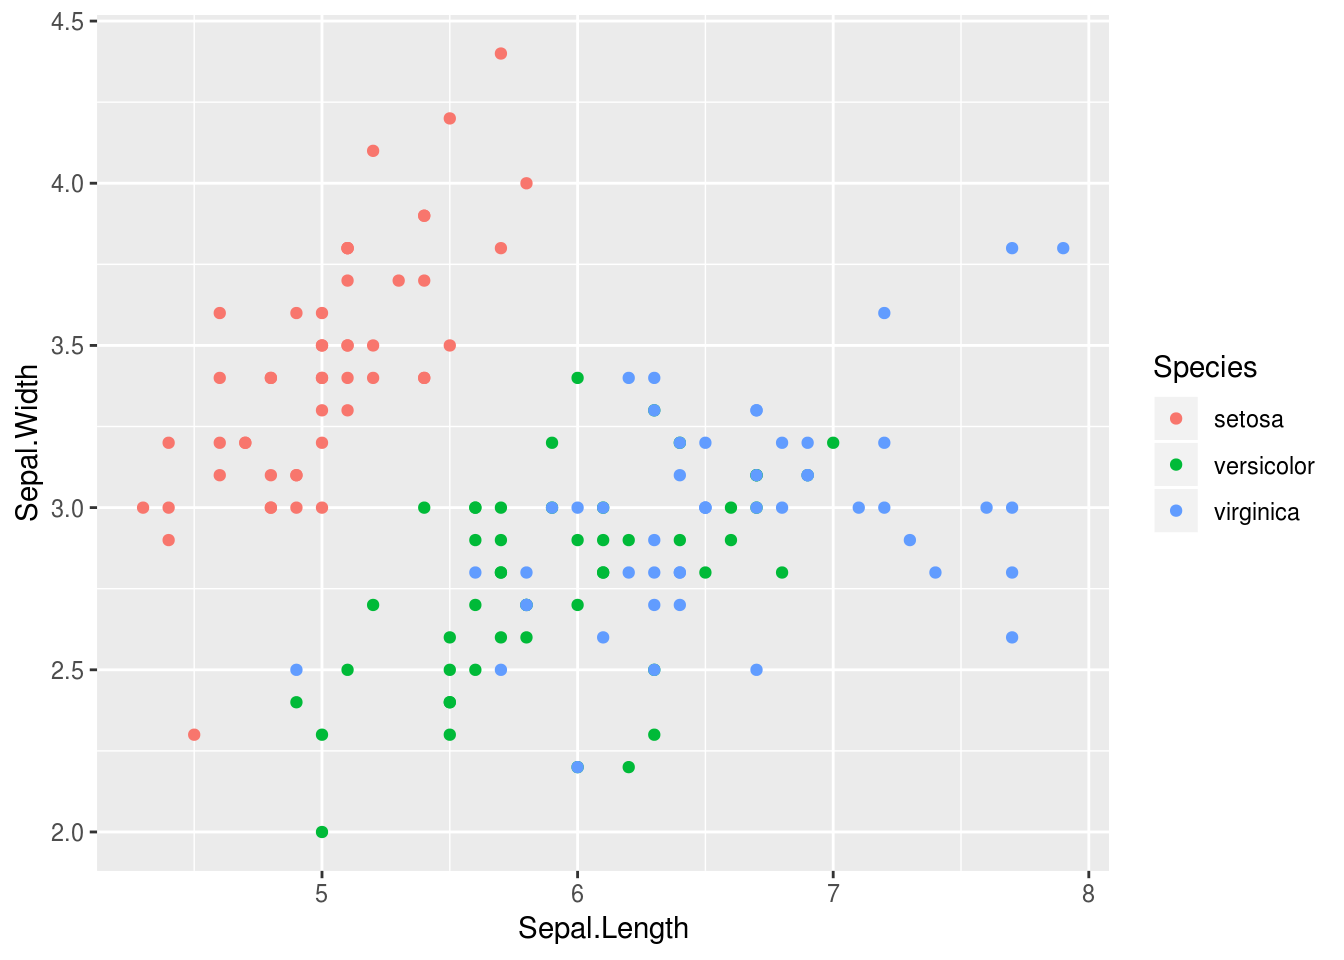
\includegraphics[width=0.7\linewidth]{ntu-bookdown_files/figure-latex/iris-1} 

}

\caption{The iris data.}\label{fig:iris}
\end{figure}

\texttt{見圖\ \textbackslash{}@ref(fig:iris)}產生:見圖 \ref{fig:iris}

\subsection{Figure Caption}\label{figure-caption}

對於比較複雜的 caption,可以使用 Text reference 的方式:

\begin{Shaded}
\begin{Highlighting}[]
\NormalTok{對於比較複雜的 caption,可以使用 Text reference 的方式:}

\NormalTok{(ref:dia) 插入**引用資料** [@kassin2017] 的 Figure Caption.}

\NormalTok{```\{r dia, fig.cap='(ref:dia)', fig.show='hold', out.width=c('48%','48%')\}}
\NormalTok{ggplot(data = diamonds) +}
\NormalTok{  geom_point(aes(x = carat, }
\BaseNTok{                 y = price,}
\BaseNTok{                 color = cut),}
\BaseNTok{             size = 0.1) +}
\NormalTok{  guides(color = guide_legend(}
\BaseNTok{    override.aes = list(size = 2)}
\BaseNTok{    ))}

\NormalTok{pl_iris # Second figure}
\NormalTok{```}
\end{Highlighting}
\end{Shaded}




\begin{figure}[H]

{\centering 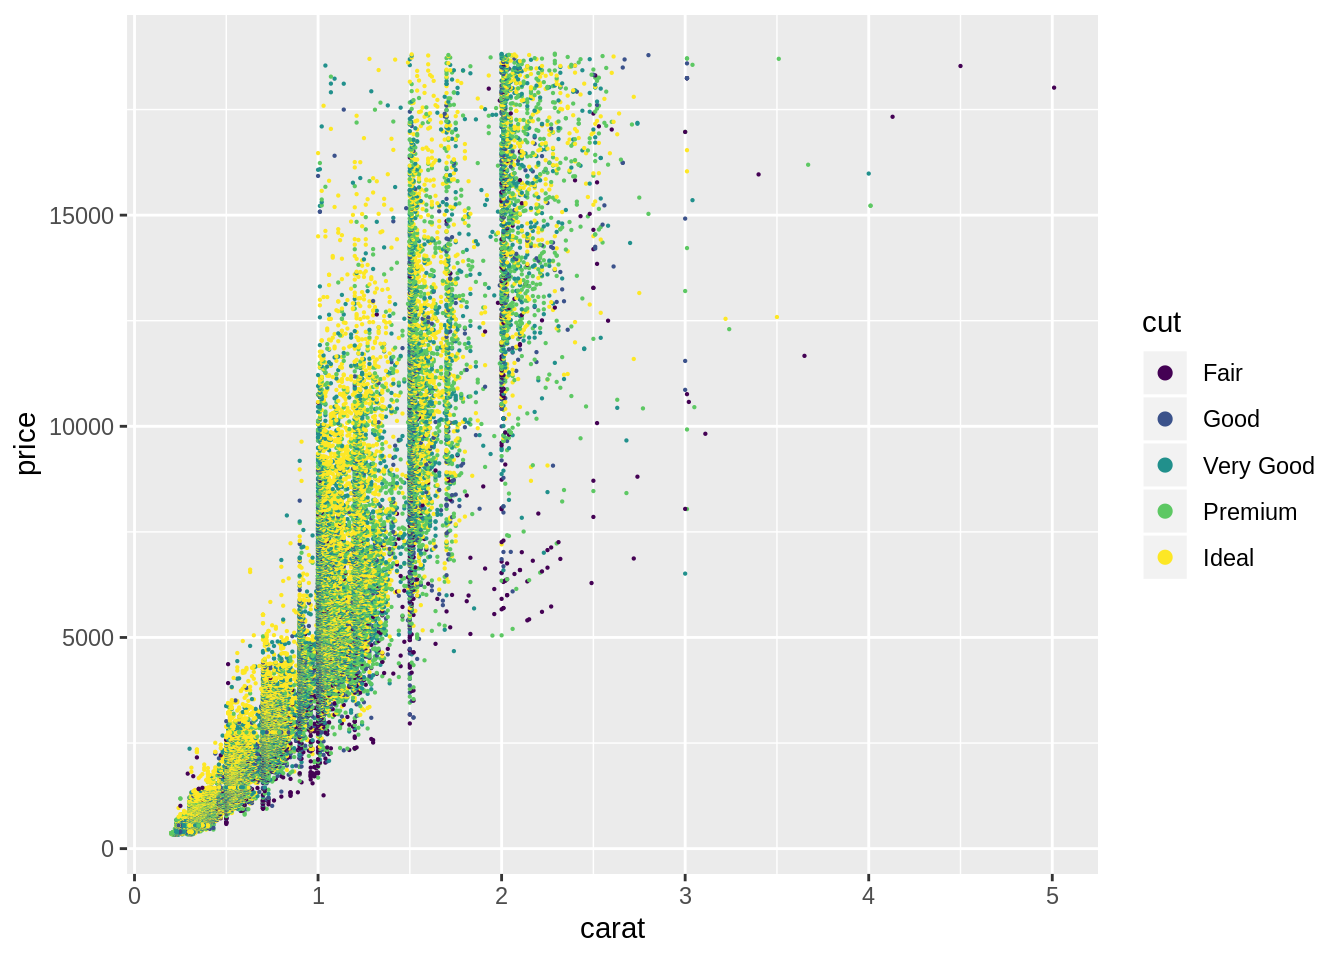
\includegraphics[width=0.48\linewidth]{ntu-bookdown_files/figure-latex/foo-1} 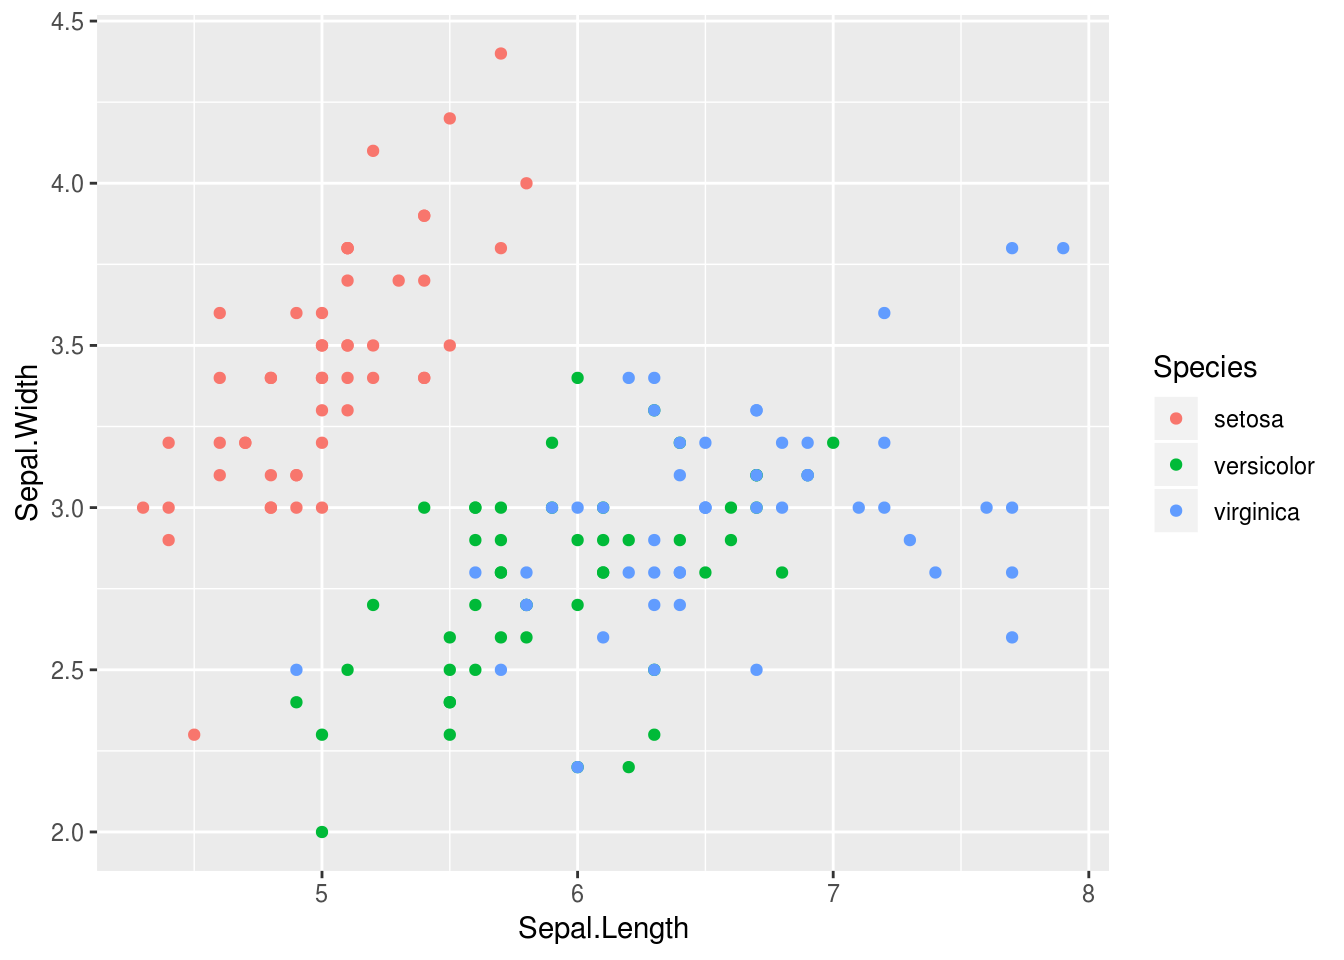
\includegraphics[width=0.48\linewidth]{ntu-bookdown_files/figure-latex/foo-2} 

}

\caption{插入\textbf{引用資料} (Kassin, Fein, \& Markus,
\protect\hyperlink{ref-kassin2017}{2017}) 的 Figure Caption.}\label{fig:foo}
\end{figure}

\section{Table Referencing}\label{table-referencing}

\begin{Shaded}
\begin{Highlighting}[]
\NormalTok{(ref:mtcars) Dynamic variable in caption: }\BaseNTok{`r Sys.time()`}\NormalTok{.}

\NormalTok{```\{r mtcars, echo=FALSE\}}
\NormalTok{knitr::kable(}
\NormalTok{  head(mtcars[, 1:8], 5), booktabs = TRUE,}
\NormalTok{  caption = '(ref:mtcars)'}
\NormalTok{  )}
\NormalTok{```}

\FunctionTok{### Link Table in Later Sections \{-\}}
\NormalTok{見表 \textbackslash{}@ref(tab:mtcars)}
\end{Highlighting}
\end{Shaded}



\begin{table}[t]

\caption{\label{tab:mtcar}Dynamic variable in caption: 2018-11-09 21:28:40.}
\centering
\begin{tabular}{lrrrrrrrr}
\toprule
  & mpg & cyl & disp & hp & drat & wt & qsec & vs\\
\midrule
Mazda RX4 & 21 & 6 & 160 & 110 & 3.9 & 2.6 & 16 & 0\\
Mazda RX4 Wag & 21 & 6 & 160 & 110 & 3.9 & 2.9 & 17 & 0\\
Datsun 710 & 23 & 4 & 108 & 93 & 3.9 & 2.3 & 19 & 1\\
Hornet 4 Drive & 21 & 6 & 258 & 110 & 3.1 & 3.2 & 19 & 1\\
Hornet Sportabout & 19 & 8 & 360 & 175 & 3.1 & 3.4 & 17 & 0\\
\bottomrule
\end{tabular}
\end{table}

\subsection*{Link Table in Later
Sections}\label{link-table-in-later-sections}
\addcontentsline{toc}{subsection}{Link Table in Later Sections}

見表 \ref{tab:mtcar}

\section{總整理}

\begin{itemize}
\tightlist
\item
  \texttt{(ref:mtcar)\ Text\ refereces}
\item
  \texttt{\textbackslash{}@ref(fig:fig-label)}

  \begin{itemize}
  \tightlist
  \item
    \texttt{fig-label} is code chunk label
  \end{itemize}
\item
  \texttt{\textbackslash{}@ref(thm:thm-label)}

  \begin{itemize}
  \tightlist
  \item
    \texttt{thm-label} is code chunk label
  \end{itemize}
\item
  \texttt{\textbackslash{}@ref(tab:tab-label)}

  \begin{itemize}
  \tightlist
  \item
    \texttt{tab-label} is code chunk label. Use text reference for
    complicated captions.
  \end{itemize}
\item
  \texttt{\textbackslash{}@ref(eq:eq-label)}

  \begin{itemize}
  \tightlist
  \item
    Defined as \texttt{(\textbackslash{}\#eq:eq-label)} in LaTeX
    equation environment
  \end{itemize}
\item
  Benefits
\item
  Quick Start

  \begin{itemize}
  \tightlist
  \item
    General Usage

    \begin{itemize}
    \tightlist
    \item
      Front matter
    \item
      Content
    \end{itemize}
  \item
    Write Thesis in English (Write in Eng)
  \end{itemize}
\item
  Resources

  \begin{itemize}
  \tightlist
  \item
    R Markdown Features
  \end{itemize}
\item
  Thanks and Help

  \begin{itemize}
  \tightlist
  \item
    GitHub issues
  \end{itemize}
\end{itemize}

\chapter{進階功能擴充}\label{add-on}

透過其它 R 套件,R Markdown
的撰寫過程能夠更順暢。以下介紹幾個例子,歡迎補充說明。

\section{語言學}\label{ling}

語言學相關文件寫作時,常需要插入 IPA
語音符號,但鍵盤通常難以直接打出這些符號。為此,我寫了一個 R
套件,讓使用者能直接在 RStudio 中透過輸入語音 features 的方式打出 IPA:

\begin{figure}[H]

{\centering 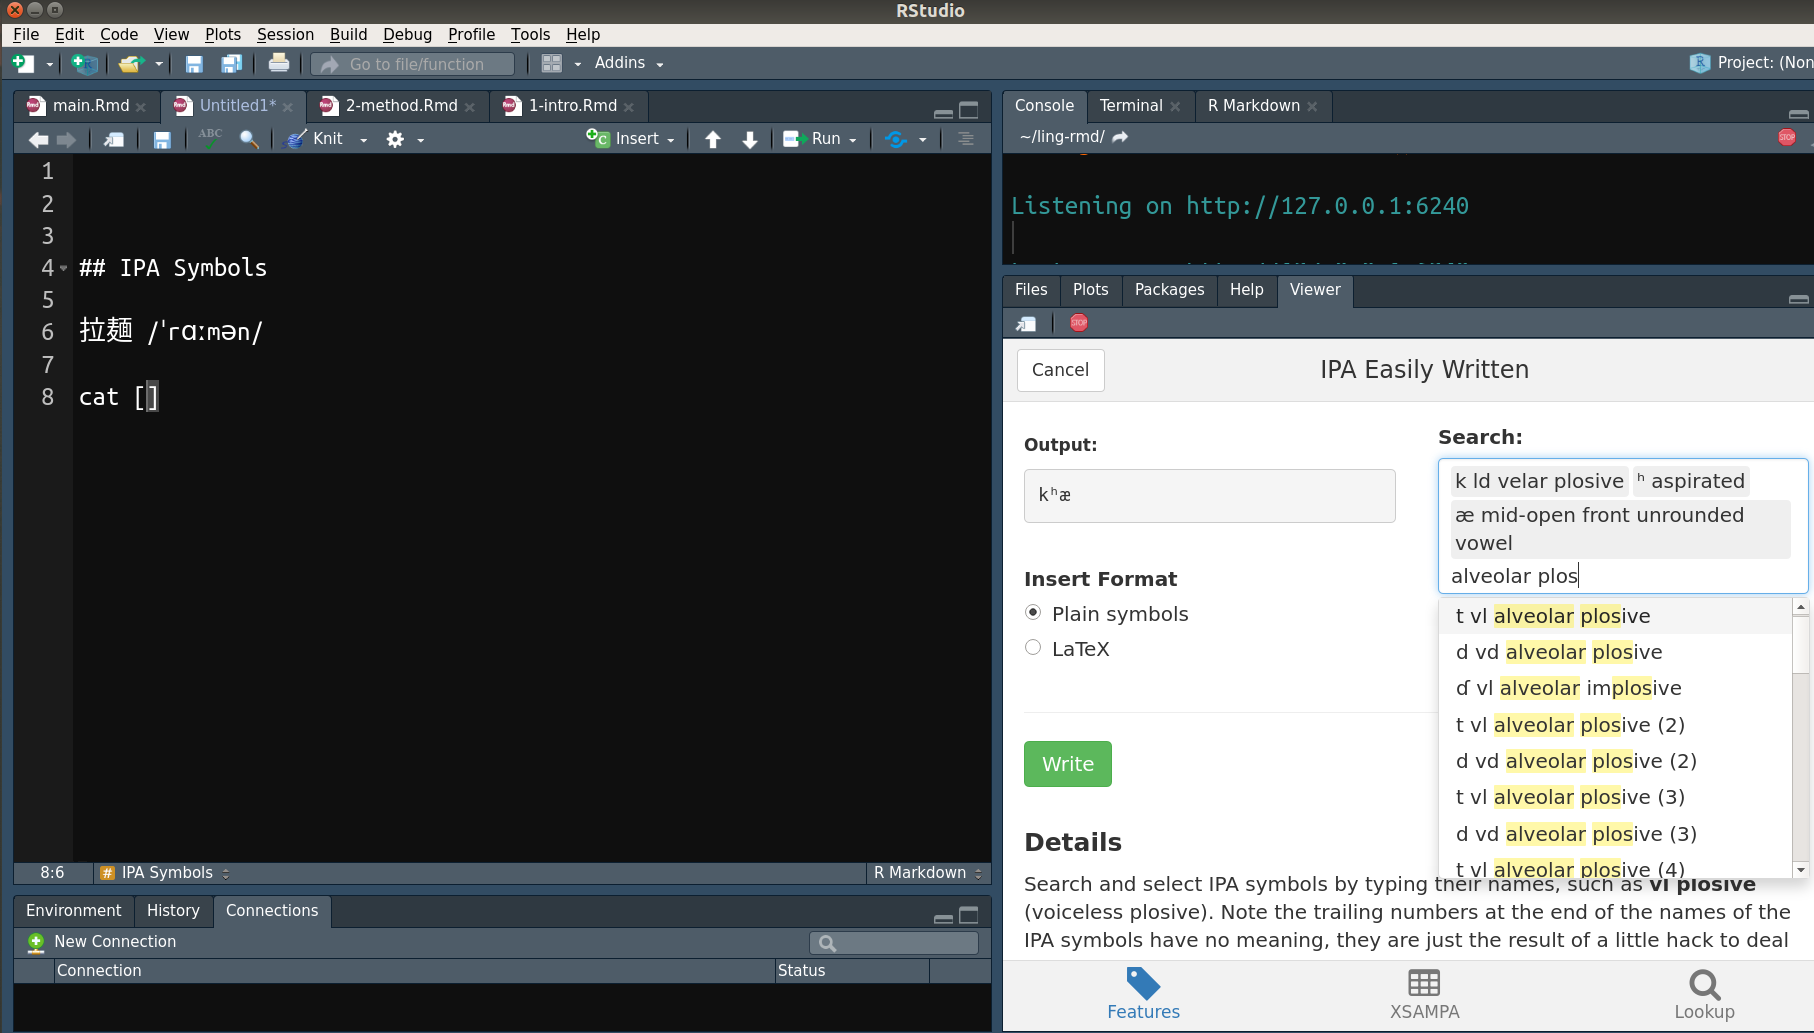
\includegraphics[width=1\linewidth]{figs/ipa} 

}

\caption{使用 linguisticsdown 套件插入 IPA 音標符號}\label{fig:unnamed-chunk-9}
\end{figure}

要使用這功能,需安裝 \texttt{linguisticsdown}:

\begin{Shaded}
\begin{Highlighting}[]
\KeywordTok{install.packages}\NormalTok{(}\StringTok{"linguisticsdown"}\NormalTok{)}
\end{Highlighting}
\end{Shaded}

並且在 \texttt{index.Rmd} 的 yaml 設定 IPA
符號專用的字型(需確認電腦上有安裝此字型):

\begin{Shaded}
\begin{Highlighting}[]
\FunctionTok{ipa-font:}\AttributeTok{ }\StringTok{'Doulos SIL'}
\end{Highlighting}
\end{Shaded}

關於更詳細的功能,見\href{https://liao961120.github.io/linguisticsdown/}{套件網頁}

\cleardoublepage

\appendix \addcontentsline{toc}{chapter}{\appendixname}


\chapter{LaTeX 文獻引用}\label{latex-cite-pkg}

R Markdown 的 PDF 輸出是透過 Pandoc 的 LaTeX 模板,因此理論上 LaTeX
可以做到的事,也可以透過 R Markdown 達成。目前的問題是

\begin{quote}
LaTeX 本身並未有支援繁體中文格式的文獻引用套件
\end{quote}

經過一段時間的搜尋,發現 biblatex
套件似乎可以定義不同的引用格式\footnote{\url{https://tex.stackexchange.com/questions/417762/different-styles-between-citations-and-bibliography}\\
  \url{https://tex.stackexchange.com/questions/377308/different-citation-styles-for-the-same-bibliography}},因此,或許可以透過定義新的標點符號,例如將原本引用格式中的\texttt{,}定義成\texttt{,}、\texttt{.}定義成\texttt{。},再透過
\texttt{.bib} 檔中的 \texttt{langid} field
辨識要使用何種引用格式。然而,由於作者本人對 LaTeX
並不熟悉,因此需要這方面高手的協助。

\renewcommand{\href}{\oldhref}

\chapter*{參考資料}\label{references}
\addcontentsline{toc}{chapter}{參考資料}

\hypertarget{refs}{}
\hypertarget{ref-kassin2017}{}
Kassin, S., Fein, S., \& Markus, H. R. (2017). \emph{Social Psychology}
(10th ed.). Boston: Cengage Learning.

\hypertarget{ref-leung2008}{}
Leung, A. K.-y., Maddux, W. W., Galinsky, A. D., \& Chiu, C.-y. (2008).
Multicultural experience enhances creativity: The when and how.
\emph{American Psychologist}, \emph{63}(3), 169--181.
\url{https://doi.org/10.1037/0003-066X.63.3.169}

\hypertarget{ref-huangxuanfan1993}{}
黃宣範. (1993). \emph{語言、社會與族群意識: 臺灣語言社會學的研究}.
臺北市: 文鶴. Retrieved from
\url{http://tulips.ntu.edu.tw:1081/record=b1285025*cht}







\end{document}
